\section{Making sense of which region of parameter space contributes `a lot' to the integral}

\newcommand{\MeV}{~\mathrm{MeV}}

As Hong Yi and I were writing up the final edits for the draft of the paper we added a comment saying that 
\begin{quote}
    ``The significance of $T = 10\MeV$ can be understood as follows: at low temperatures, the thermal factors in the integrand restricts the phase space to a region where the typical momentum transfer is bigger than the screening scale; at higher temperatures, particles start to become nondegenerate so there is support near the region where $k^2=0$ in the photon propagators, where the screening effect becomes crucial.''
\end{quote}
We are motivated to make a comment like this because we needed to explain why we had to account for medium effects when we extended our numerical integration method to high temperatures. 
A chronological account of what happened goes like this:
\begin{enumerate}
    \item I tried dialing up the temperature $T$ from $T = 0.083\MeV$ to $T = 83\MeV$ without accounting for the electromagnetic screening effect arising from the background of free charged particles.
    \item I found that by neglecting this effect, the emissivity I computed was diverging. This manifested as a sharp rise in the emissivity at around $T \sim 1 \MeV$ as seen in \fref{fig:divergent-emissivity-vs-temperature}. 
    I further checked that if I increased $N_{\mathrm{eval}}$, the value of the integral would continue to increase as the numerical integrator finds points close and closer to the $1 / k^2$ pole in the matrix element. This is shown in \fref{fig:divergent-emissivity-vs-neval}.
    \begin{figure}[htbp]
        \centering
        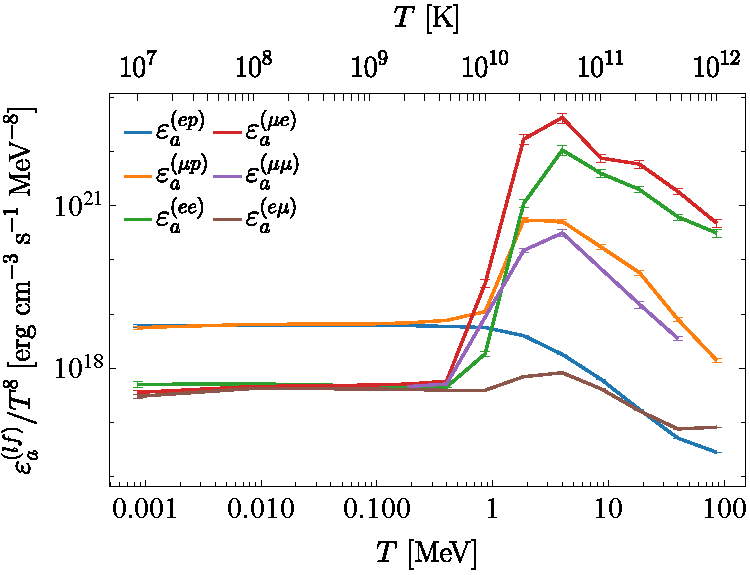
\includegraphics[width=0.5\linewidth]{figs/divergent-emissivity-vs-temperature.pdf}
        \caption{Axion emissivity, calculated without taking into account plasma screening, vs temperature. Notice that the dramatic jump in emissivity seen at $T \sim 1 \MeV$. The axion emissivity is normalized by $T^8$ since we are also interested in deviations from $T^8$ scaling -- the expected behaviour assuming the Fermi surface approximation.}
        \label{fig:divergent-emissivity-vs-temperature}
    \end{figure}
    \begin{figure}[htbp]
        \centering
        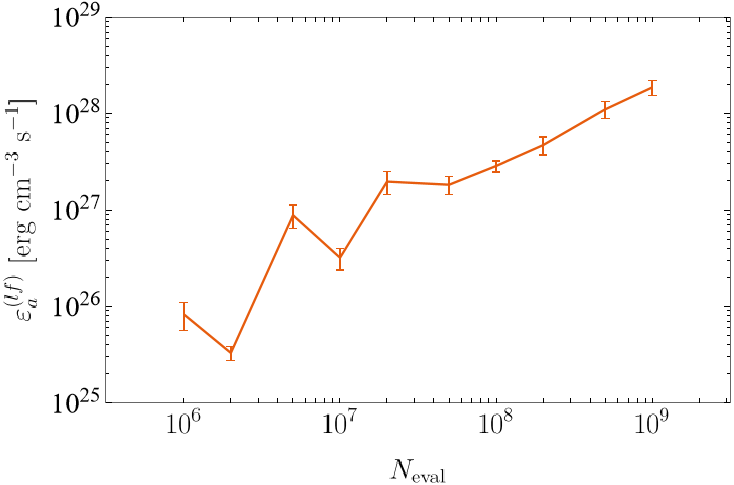
\includegraphics[width=0.5\linewidth]{figs/divergent-emissivity-vs-neval.png}
        \caption{$\varepsilon_a^{(\mu e)}$, calculated without taking into account plasma screening, vs $N_{\mathrm{eval}}$. $T = 4 \MeV$, $\beta_{F,\mu} = 0.84$, $m_a = 0$, $n = 10$. If the integral was converging this plot should approach a constant as $N_{\mathrm{eval}}$ is increased. Instead, we observe that $\varepsilon_a^{(\mu e)}$ increases without bound.}
        \label{fig:divergent-emissivity-vs-neval}
    \end{figure}
    \item Based on the observations in the previous point we surmised that at low temperatures the exponential suppression from the thermal factors prevented my numerical integrator from running into trouble at the pole where $k^2 = 0$. I can check this by sampling points in the integration domain using my trained numerical integrator and checking if there were any points I ran into where $k^2$ was very close to zero.
    \item We realised that we needed to account for plasma effects and ended up doing so by making the replacement  $k^{-2} \rightarrow (k^2 + k_{TF}^2)^{-1}$ in the photon propagators in the matrix element. This gave us a finite emissivity that converged. We believe this is sufficient evidence for the claim that the $k^{-2}$ pole was the problem leading to diverging emissivities.
\end{enumerate}